\documentclass[11pt,reqno]{amsart}
%%% WARNING: Do NOT change the page size, fonts, or margins!  Penalties will apply.


\usepackage{graphicx}
\usepackage{amssymb,amsmath,amsthm, amsmath, amsthm, amscd, amsfonts, amssymb, graphicx, color}
\usepackage{placeins} %enables \FloatBarrier, that prevents floats from going below it.


%%% WARNING: Do NOT change the page size, fonts, or margins!  Penalties will apply.
%%% WARNING: Do NOT change the page size, fonts, or margins!  Penalties will apply.

\newtheorem*{remark}{Remark 1.1}

\begin{document}

\title{The Simeoni Model for Tumor Growth}
\author{Sophie Carter, Morgan Nielsen, Michelle Wang, Sarah Winters}
\date{November 21, 2023}

%% comment out next command to put today's date after names of group members, or put a desired day in the parethesis


\maketitle

\begin{abstract}
The Simeoni Model is a system of ordinary differential equations that represents tumor growth as it receives different treatments. After researching the constants, variables, and functions used in this model, we created graphs to see how changing the parameters affected the model and what it implied about tumor growth. We conclude that this model successfully represents immunotherapeutic and chemotherapeutic treatment on tumor cells, and we are curious about how the different constants are related to the various cancer treatments. 
\end{abstract}

%% First Section
\section{Background/Motivation}
As a team, our search for a suitable situation or phenomenon to model encountered some obstacles. Initially, many concepts we considered were better suited for a Partial Differential Equation (PDE) rather than an Ordinary Differential Equation (ODE), which we aimed to avoid based on advice from our professor. Additionally, we sought a topic with a significant impact on people's lives. This led us to focus on analyzing the Simeoni Model (1.1), specifically its application in modeling cancerous tumor growth within the body \cite{Koziol_Falls_Schnitzer_2020}.

\begin{equation}\label{eq:1.1}
\begin{aligned}
    \frac{dZ_1}{dt} &= TGF(t) - k_1c(t)Z_1(t), \\
    \frac{dZ_2}{dt} &= k_1c(t)Z_1(t) - k_2Z_2(t), \\ 
    \frac{dZ_3}{dt} &= k_2Z_2(t) - k_2Z_3(t), \\
    \frac{dZ_4}{dt} &= k_2Z_3(t) - k_2Z_4(t)
\end{aligned}
\tag*{(1.1)}
\end{equation}
\hspace{2em}

Cancer is a complex group of diseases characterized by the uncontrolled division and growth of abnormal cells, which can infiltrate and destroy normal tissues within the body. Tumor growth, a hallmark of cancer, poses a critical threat as it can lead to the disruption of essential physiological processes by cutting off the oxygen and nutrient supply to surrounding tissues \cite{Cancer_Research_2023}. As cancer progresses, it often metastasizes, spreading to other parts of the body and compounding the challenges of treatment. The profound impact of cancer on individuals' lives, coupled with the urgent global quest for improved solutions and treatments, underscores the importance of studying and modeling tumor growth.

Our motivation for selecting the Simeoni Model as the focus of our research stems from its application in addressing the intricate dynamics of cancerous tumor growth within the body. By delving into this modeling framework, we aim to contribute to existing research efforts seeking to better understand solutions and treatments for cancer. The Simeoni Model provides a valuable platform for simulating and understanding the intricate processes involved in tumor development. Analyzing and modifying this model can offer insights into the underlying mechanisms of cancer progression, potentially leading to more effective strategies for intervention and treatment. Ultimately, our research endeavors aspires to contribute to the broader goal of preventing the devastating consequences of uncontrolled tumor growth and, in turn, improving the prognosis and quality of life for individuals facing cancer diagnoses.


%% Second Section 
\section{Modeling}
Though they're not representing the same things, part of our interest in the Simeoni Model was from the similarities it has to the SIR Model. This model surrounds the idea of the tumor cells moving from one compartment to another; these compartments are represented by the four functions $Z_1(t)$, $Z_2(t)$, $Z_3(t)$, and $Z_4(t)$. Similarly to the basic SIR Model with constant rates representing the change from one state to another, this system looks at how the tumor cells damaged by treatment are moving to the next compartment. The sum of the cells in each of the four compartments represents the total volume of the tumor. The first compartment $Z_1$ is the model of the growth of the tumor before it is damaged by treatment, so this includes both the change of cells moving from $Z_1$ to $Z_2$ and the growth function of the tumor itself. In our model, moving from one compartment to another represents the tumor weakening; the tumor cells in the $Z_4$ compartment are those most affected by medical treatment, and are therefore the closest to elimination. 

After defining the distinct compartments, we will define the constants and growth function integral to the Simeoni model. As discussed earlier, the $Z_1$ compartment signifies the actively growing segment of the tumor, the stage farthest away from cell elimination. This cell growth is governed by the Tumor Growth Function, denoted as $TGF(t)$ \ref{eq:1.2}, which evolves dynamically over time. Concurrently, $c$$($$t$$)$ induces a fraction of tumor cells to undergo programmed cell death, guided by a killing constant 
$k_1$, thereby transitioning these cells to a higher compartment. Along with $k_1$,  the tumor cells sustain continual damage at a consistent rate of $k_2$ and are relocated to compartment $Z_3$ or $Z_4$. \cite{Koziol_Falls_Schnitzer_2020}.


\begin{equation} \label{eq:1.2}
\begin{aligned}
    TGF(t) &= \frac{\lambda_0Z_1(t)}{[1 + (\frac{\lambda_0}{\lambda_1}V(t))^\psi]^\frac{1}{\psi}}, 
\end{aligned}
\tag*{(1.2)}
\end{equation}
\qquad where $V(t)$ is the total tumor volume, $\lambda_0$, $\lambda_1$, and $\psi$ are constants. The constants' meaning are not listed in the model. 

\begin{remark}
    The parameters $\lambda_0, \lambda_1$, and $\psi$ were not explicitly discussed too much in our sources of research on the Simeoni Model. However, changing these constants can have tumors die completely, which could be considered in our final conclusions.
\end{remark}


Various techniques and methods have been historically employed to tackle the challenge of modeling tumor growth and decay. Prior studies have explored models such as Mendelsohn, Exponential, Linear, Logistic, and Bertalanffy, among others \cite{Murphy_Hope_2016}. Each of these models brings a unique perspective to the understanding of tumor dynamics. While Simeoni is one of the models in this repertoire, we recognize the importance of critically evaluating its suitability and effectiveness compared to alternative models.

Our pursuit into the intricacies of the Simeoni model is motivated by a fundamental question: Is the existing Simeoni model an accurate approximation for the decay/growth of tumor cells, or are there adjustments that could enhance its precision in characterizing this phenomenon? By delving into this inquiry, we aim to contribute valuable insights to the field of tumor modeling and treatment efficiency.

Our analysis goes beyond a mere comparison between models; we endeavor to comprehensively understand the intricacies of the Simeoni model and its counterparts. This involves a detailed examination of the mathematical formulations, underlying assumptions, and empirical implications of each model. By doing so, we not only position our exploration within the broader context of existing research but also aim to uncover nuances that might have been overlooked.

In response to the valuable feedback received during the proposal stage, our approach is designed to showcase a deep understanding of the subject matter. This understanding is not confined to the isolated examination of the Simeoni model but extends to a holistic appreciation of how our exploration fits into the larger landscape of tumor modeling. By elucidating the strengths and limitations of various models and synthesizing this information, our study aspires to provide a nuanced evaluation of the Simeoni model's efficacy in capturing the intricacies of tumor decay.

In doing so, we seek to make meaningful contributions to the ongoing discourse in the field, shedding light on potential adjustments to existing models and advancing our understanding of tumor behavior. This endeavor holds the promise of influencing not only theoretical aspects of tumor modeling but also practical implications for treatment strategies and therapeutic interventions.



Before adjusting the Simeoni model, we first wanted to examine its equilibria and the stability of the system at each equilibrium. An initial look at the system of ODEs shows that there is an equilibrium when each $Z_i = 0$. This occurs at $t=0$ and , so we have $Z_1(0) = Z_2(0) = Z_3(0) = Z_4(0)$. To confirm that this was the only equilibrium, we created a \verb!numpy! array representing the system, and calculated the null space. This proved that for the original Simeoni model, there is one equilibrium at the origin. In order to examine the stability of the origin, we calculated the eigenvalues of the matrix representing the model, corresponding to each $Z_i = 0$. If we use $k_1 = 0.4$, $k_2 = 0.5$, $c(t) = 0.5$, and $TGF(t) \approx 0.075$, our eigenvalues are $\lambda_1 = -0.5$, $\lambda_2 = -0.5$, $\lambda_3 = -0.5$, and $\lambda_4 \approx -0.125$. Since these values are all less than zero, we found that the origin is a stable equilibrium. Figure \ref{fig:1} is a visual representation of the model where the stability was found.
\begin{figure}[h]

\begin{center} %Put your images in a figure like this
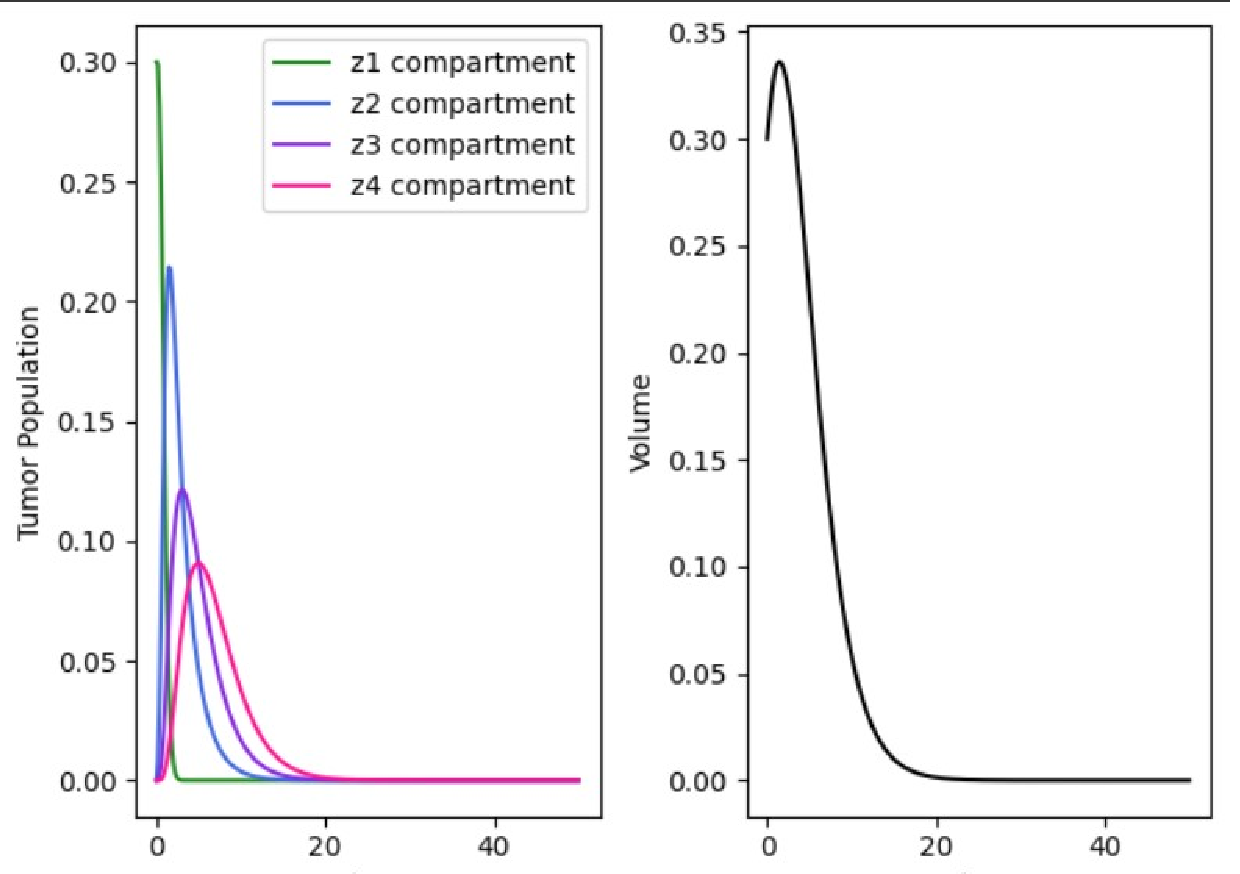
\includegraphics[width=\textwidth]{original_tumor_random_parameters.pdf}. % Better to make them pdfs than png or gif or jpeg
\end{center}
\caption{Our altered-parameters-valued model with parameters $\lambda_0=.5, \lambda_1=.2, \psi=.5, k_1 = .4, k_2=.5, c=t, V_0 = .3$}
\label{fig:1}
\end{figure}
%we should change this model (figure 1) to have the same initial volume V0 as our realistic model for consistency - michelle

To observe the tumor growth represented by the Simeoni model, we used \verb!python! to create our system of ODEs (1.1), and  \verb!matplotlib! to create the graphs, with constants that felt appropriate for the information we were given. We solved our IVP with Scipy \verb!solve_ivp!, and then plotted these solutions to observe each compartment's behavior. This is a non-linear model, since the system of differential equations includes functions like the Tumor Growth function (1.2) as a function of $Z1$ and the sum of $Z1$, $Z2$, $Z3$, and $Z4$, which constitute the volume. The model consists of constant parameters, including $k_1$, $k_2$, $\lambda_0$, $\lambda_1$, and $\psi$. We found that the values of these constant parameters that model the tumor growth most realistically and similarly to existing research \cite{Koziol_Falls_Schnitzer_2020} are those that are smaller than $0.5$ and greater than $0$. See figure \ref{fig:2} for a visual representation for that model. 
\begin{figure}[h]
\begin{center} %Put your images in a figure like this
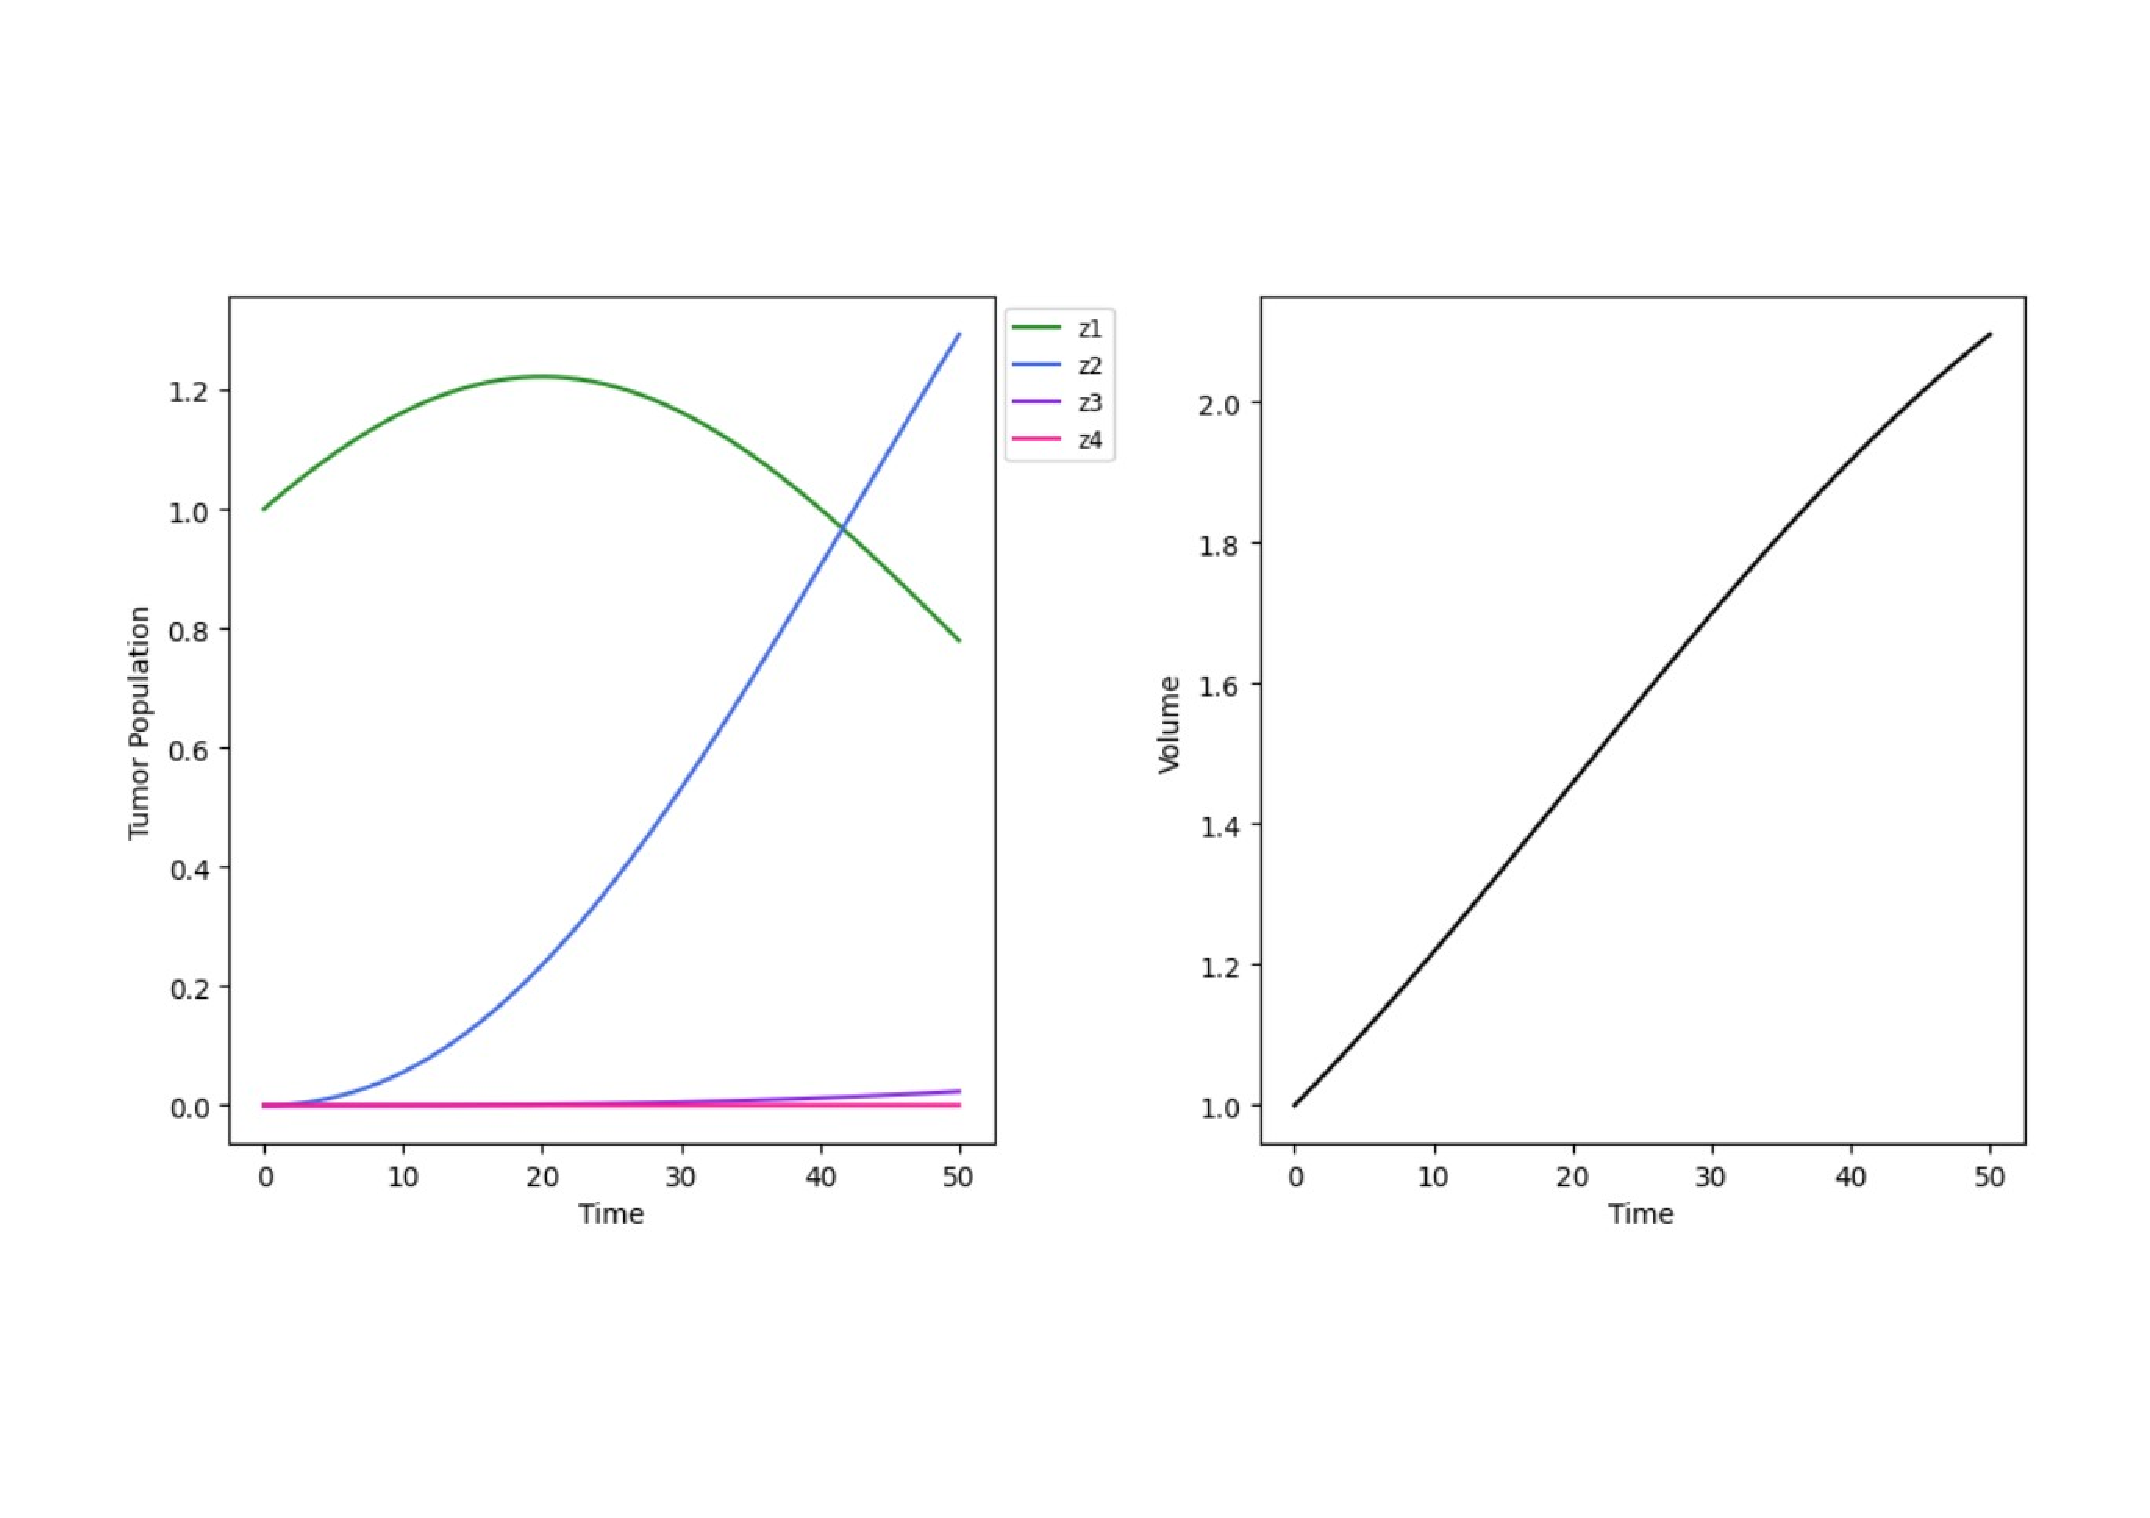
\includegraphics[width=\textwidth]{parameters_like_paper.pdf}. % Better to make them pdfs than png or gif or jpeg
\end{center}
\caption{Realistic valued model, with parameters: $\lambda_0=0.02, \lambda_1=0.001, \psi=-2, c=t, k_1=0.001, k_2=0.001, V_0=1$}
\label{fig:2}
\end{figure}

Within the Simeoni Model, the parameter c(t) represents the concentration of a chemotherapeutic or immunotherapeutic agent in the Z1 compartment at time t. Therefore, allowing for c(t) to equal zero at all values of t gives us tumor growth in the absence of any treatment. Figure \ref{fig:3} plots untreated tumor growth against time. Compare with Figure \ref{fig:2}, which has the same given parameters. It is worth noting that we do observe what we would expect to observe. Under the same given parameters, there is higher tumor volume over time in the absence of treatment than there is under treatment.

\begin{figure}[h]
\begin{center} %Put your images in a figure like this
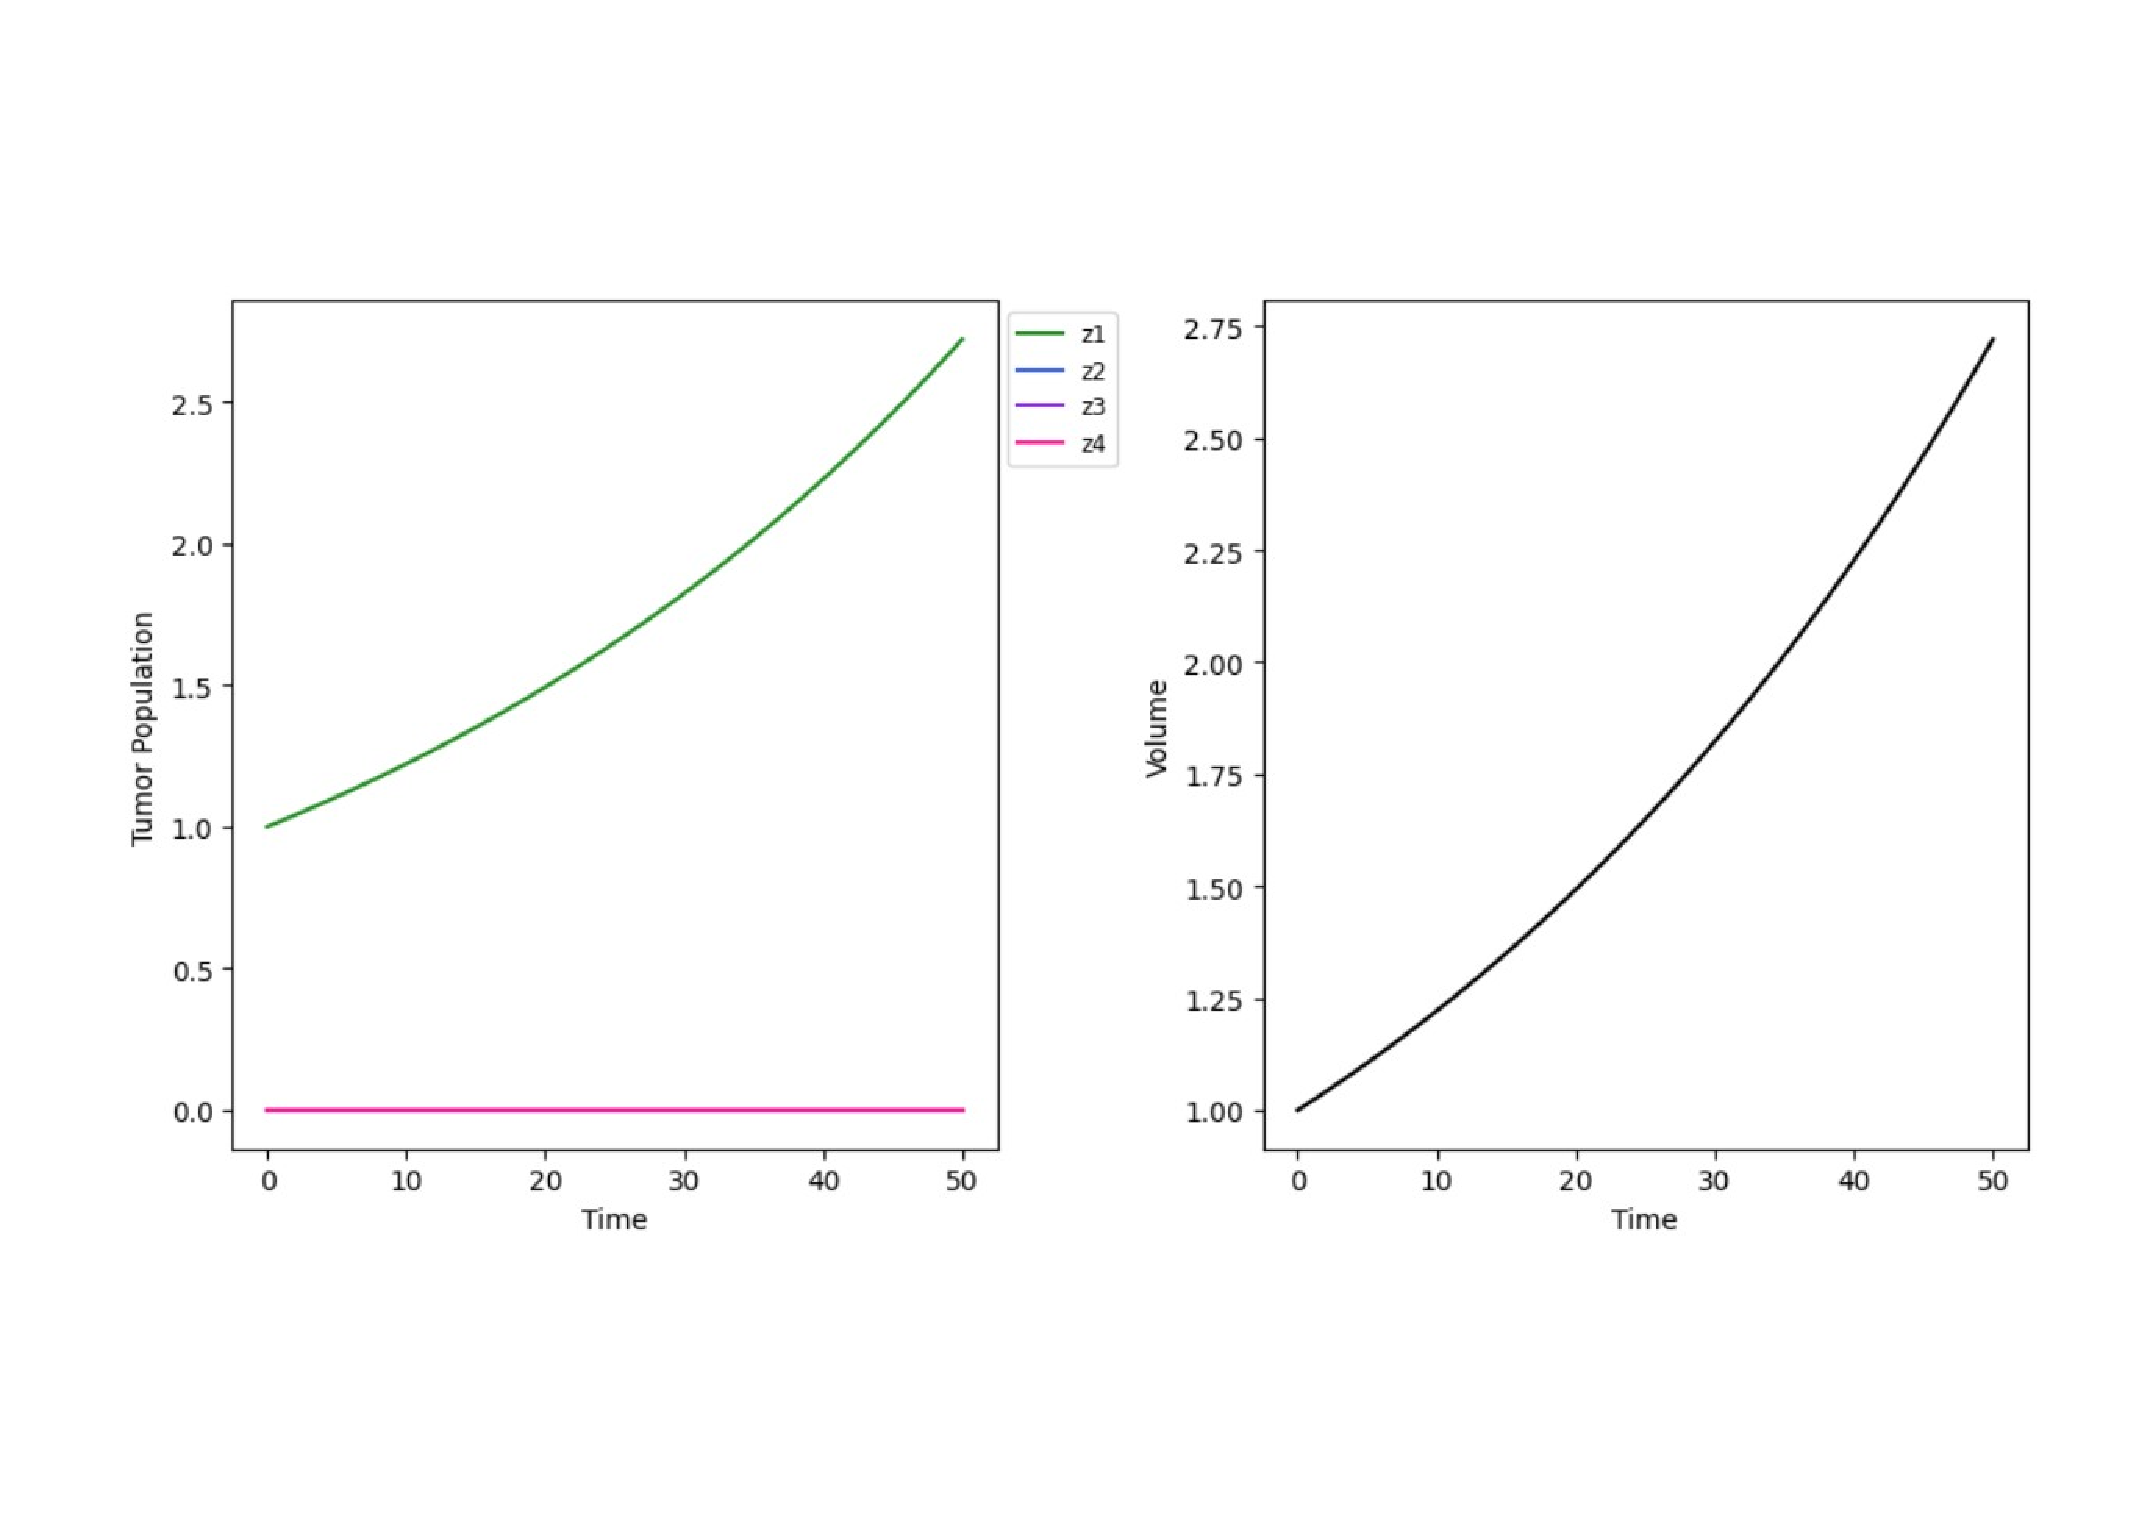
\includegraphics[width=\textwidth]{parameters_like_paper_no_treatment.pdf}. % Better to make them pdfs than png or gif or jpeg
\end{center}
\caption{Realistic valued model, with no treatment}
\label{fig:3}
\end{figure}

To further understand the model's behavior, we conducted deep parameter tuning on the constant parameters. As we tweaked each parameter we realized that this could lead to investigating the impact of each particular parameter on the efficacy of chemotherapy and immunotherapy. Our model's behavior prompted us to explore various parameter combinations, ultimately leading to surprising discoveries. Initially, as we are not cancer experts, we did not know how a "normal" cancer model should behave, and the intricacies of each parameter's influence were not well understood. 
%this paragraph above seems kind of repetitive; in particular, the first few sentences - michelle

In order to understand each constant parameter's influence better, we varied these parameters to observe their effects on the cancer population over time. When each constant parameter is increased relative to the constant parameter setting of the realistic model, we find that tumor growth increases at a slower rate. With parameter values high enough, the overall tumor volume even eventually returns to zero, signifying a state void of any remaining tumor cells. This potentially has very significant implications: if the constant parameters can be realistically manipulated to reach the values as in our altered model, the same levels of chemotherapeutic and immunotherapeutic treatment will yield much more effective outcomes. 


Figure \ref{fig:1} and Figure \ref{fig:4} illustrate the rapid decrease of tumor volume upon increasing the values of the constant parameters. With specific parameter values as outlined in the respective captions, we find that we can not only slow tumor growth rate but also completely eradicate all tumors. As seen in Figure \ref{fig:1}, all tumors are essentially gone within 20 days.

\begin{figure}[h]
\begin{center} %Put your images in a figure like this
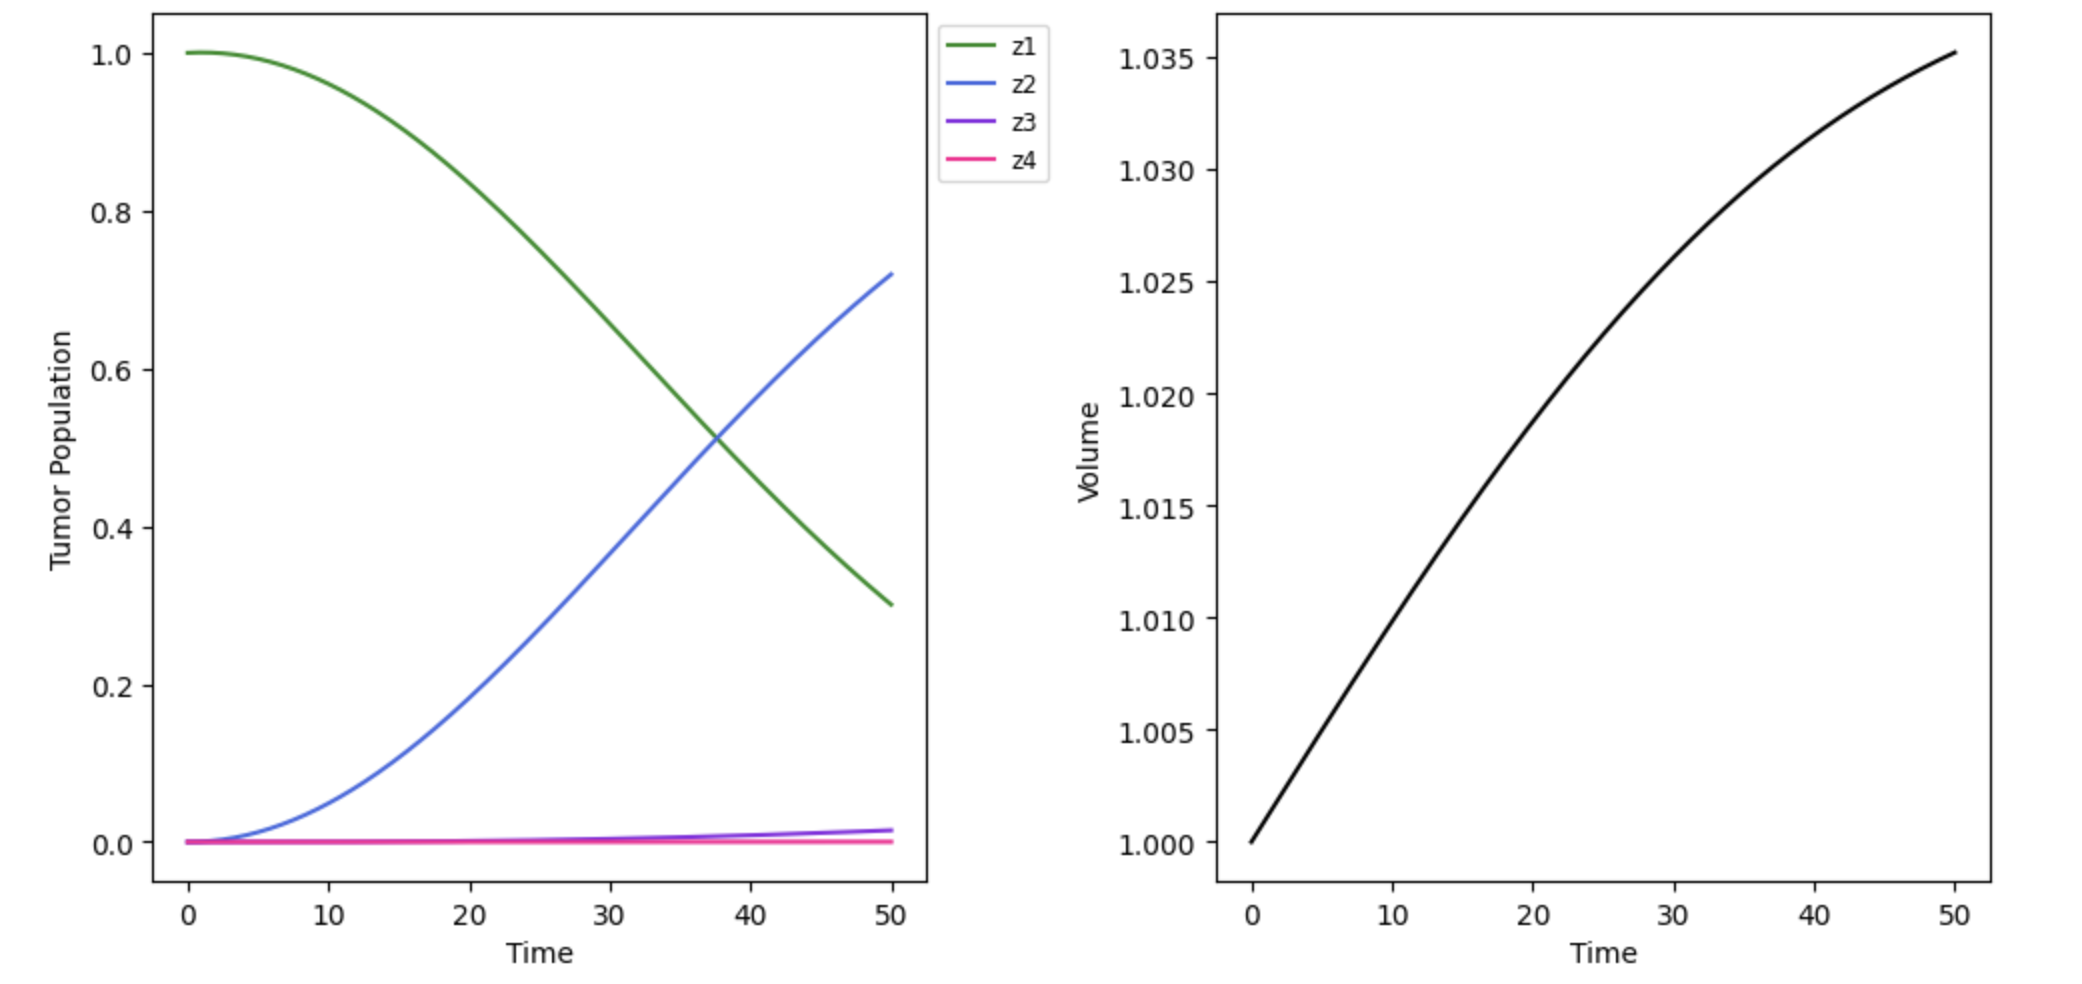
\includegraphics[width=\textwidth]{altered.png}. % Better to make them pdfs than png or gif or jpeg
\end{center}
\caption{Our altered-parameters-valued model with parameters $\lambda_0=0.02, \lambda_1=0.001, \psi=2, k_1 = 0.001, k_2=0.001, V_0 = 1$}
\label{fig:4}
\end{figure}

% should check if our realistic model is truly similar to what the research says; either way though we can slow tumor growth rate by increasing parameters




%% Third Section
\section{Results}
%Talk about how if we can build a cancer treatment to model this it would be great!
 We believe that our model can accurately describe some tumor growth, but can be affected by changing the parameters. In order to find the accuracy of our model we would need to conduct further investigation and validation in medical testing. It is important to explore the feasibility of directly manipulating these parameters in real-world scenarios and to determine the optimal combination for achieving the most effective cancer treatment. 

%%Fourth Section
\section{Analysis/Conclusions}
The Simeoni model realistically reflects the chemotherapeutic and immunotherapeutic treatment on tumor growth. In the absence of such treatment agents, tumor growth is increased. Increasing the constant parameter values in the Simeoni model results in slower tumor growth rates and even, in some cases, complete annihilation of all existing tumors. Should it be realistically possible and ethical to attain such values for the constant parameters as in our altered models, the efficacy of the same levels of chemotherapeutic and immunotherapeutic agents can be greatly increased. Nonetheless, these findings suggest that even minimally increasing the values of the constant parameters can have positive effects on slowing tumor growth.
%can do more to find out what is the minimum to increase (statistically significant) to have a meaningful effect on slowing tumor growth


We intend to explore and dissect the Simeoni model further by next altering the c(t) function. Findings from these particular alterations can lend insight into optimal amounts of chemotherapeutic and immunotherapeutic agent concentrations at different times. We also intend to experiment with different initial values of Z1, which can lend valuable insight into efficacy of treatment at earlier vs later and slower vs rapid onset stages of cancer.
%SEE COMMENT FOR THIS PARTICULAR PARAGRAPH%
%This is just for the final draft. This is something we will actually do and write up for the final final project. So this is just a placeholder until we have those models completed.

% Should probably add an errors or things affecting our findings paragraph. And then a real paragraph for further research.

% \begin{figure}[h]
% \begin{center} %Put your images in a figure like this
% \includegraphics[width=\textwidth]{Myfig.pdf}. % Better to make them pdfs than png or gif or jpeg
% \end{center}
% \label{fig:MatrixError}
% \end{figure}





%%%%%%%%%%%%%%%%%%%%%%%%%%%%%%%%%%%%%
%% Bibliography below
%%%%%%%%%%%%%%%%%%%%%%%%%%%%%%%%%%%%%
\FloatBarrier % Keep the figures from being put after the bibliography
\newpage
%% If using bibtex, leave this uncommented
\bibliographystyle{plain}
\bibliography{refs}{} %if using bibtex, call your bibtex file refs.bib

%% If not using bibtex, comment out the previous two lines and uncomment those below
%%\begin{thebibliography}{99}
   %% \bibitem{article}
     %%   Koziol, J.A., Falls, T.J. & Schnitzer, J.E. Different ODE models of tumor growth can deliver similar  results. BMC Cancer 20, 226 (2020). https://doi.org/10.1186/s12885-020-6703-0
    %%\bibitem{article}
     %%   Murphy, H., Jaafari, H. & Dobrovolny, H.M. Differences in predictions of ODE models of tumor growth: a cautionary example. BMC Cancer 16, 163 (2016). https://doi.org/10.1186/s12885-016-2164-x
%%\end{thebibliography}

\end{document}